\documentclass[10pt,aspectratio=169]{beamer}
\usepackage{preamble}
\usetheme{metropolis}
\usepackage{appendixnumberbeamer}
\usepackage{animate}
\usepackage{media9}
\usepackage{listings}
\usepackage[export]{adjustbox}
\lstset
{
    language=[LaTeX]TeX,
    breaklines=true,
    basicstyle=\tt\scriptsize,
    keywordstyle=\color{blue},
    identifierstyle=\color{magenta},
}
\title{Getting Started with \text{\LaTeX}}
\subtitle{And why I don't use Word anymore}
\date{\today}
\author{Jack Naylor}
\institute{Casual Academic - University of Sydney\\ President - MUGS (2019)}
\titlegraphic{\hfill\includegraphics[height=3.5cm]{mugs.png}}
\begin{document}

\maketitle
\section{What is \text{\LaTeX}?}
\begin{frame}{A bit of Background}
    \begin{itemize}
\item Widely regarded as the standard typesetting method for academic journals
\begin{itemize}
\item Far easier to present data, equations
\item Much easier to cite references (i.e. automatic footnotes, hyperlinking etc.)
\item Separates content from the formatting of documents
\end{itemize}
\onslide<2->\item Far more control over many aspects of the document
\begin{itemize}
\item Backend rather than frontend (e.g. Word)
\item Images won't disappear when moved slightly
\begin{itemize}
\item Everything is where you tell it to be
\end{itemize}
\end{itemize}
\end{itemize}
\end{frame}
\begin{frame}
\begin{itemize}
\item Files can be as big as needed, don't need to worry about a 30+ page Word doc crashing
\item Multi-file documents are very easy to achieve, no post-processing
\item It looks \alert{pretty}
\end{itemize}
\end{frame}
\begin{frame}
\centering
Something to keep in mind throughout this presentation: \emph{\alert{every single slide} is done in \LaTeX}
\end{frame}
\section{What can I do?}
\begin{frame}
\centering
    In short: anything you can do with Word + much much more!!
\end{frame}
\begin{frame}{Images}
   \begin{figure}
\centering
\includegraphics[width=\textwidth]{ariba}
\end{figure}
\end{frame}
\begin{frame}
Diagrams from scratch:
\begin{figure}[H]
  \centering
  \resizebox{0.9\textwidth}{!}{\begin{tikzpicture}
  
\draw[<->] (6.5,6) -- (6.5,3);
\draw[<->]  (5.5,6) -- (5.5,3);
\node[above] at (6.5,6) {\Huge{E}};
\node[above] at (5.5,6) {\Huge{F}};

\draw (-9.125,-0.5) -- (-10.125,-1) -- (-9.125,-1.5);
\draw  plot[smooth, tension=.7] coordinates {(-9.625,-0.75) (-9.5,-1) (-9.625,-1.25)};
\node at (-9.625,0) {\Huge{Camera}};

\node[rotate=-90] at (19.5,4.5) {\Huge{Object}};
\draw[blue,dashed,postaction={on each segment={mid arrow=blue}}] (20,6) node (v2) {} -- (6.5,3.75) -- (5.5,3.75) -- (2,3) node (v1) {};
\draw[blue,dashed,postaction={on each segment={mid arrow=blue}}] (v2) -- (5.5,4.375) -- (v1);
\draw[blue,dashed,postaction={on each segment={mid arrow=blue}}] (v2)  -- (6.5,5.5) -- (5.5,5.25) -- (v1);
\draw[->,thick,] (20,2.5) -- (20,6.5);
\draw[red,dashed,postaction={on each segment={mid arrow=red}}] (20,3) node (v3) {}  -- (6.5,3.75) -- (5.5,4) -- (1.5,4) node (v4) {};
\draw[red,dashed,postaction={on each segment={mid arrow=red}}] (v3) -- (5.5,4.625) -- (v4);
\draw[red,dashed,postaction={on each segment={mid arrow=red}}] (v3) -- (6.5,5.5) -- (5.5,5.5) -- (v4);

\draw[->,thick] (1.5,4) node (v7) {} -- (2,3) node (v5) {};
\draw[dotted] (-9.5,-1) node (v6) {} -- (v5);
\draw[dotted] (v6) -- (v7);
\node at (1.5,5) {\Huge{Image}};
  \end{tikzpicture}}
  \caption{Image formation captured by imaging camera}
  \label{fig:my_label}
\end{figure}
\end{frame}
\begin{frame}
GIFS:
    \begin{figure}
\animategraphics[loop,autoplay,scale=1]{7}{elon/new-}{0}{76}
\end{figure}
\end{frame}
\begin{frame}
\centering
    \includegraphics[width=\textwidth]{oohyeah}
\end{frame}
\begin{frame}{Maths}
\begin{itemize}
    \item Inline:\\
    It is known that $y=x^2+2x+4$ is a parabola.\par
    \item Block:\\
    Here is a Fourier transform:
    \[\mathcal{F}\left(\omega\right)=\int_{-\infty}^\infty f(t) e^{i\omega t}\dd t\]
    \item Numbered:
    \begin{subequations}
    \begin{align}
        \ket{+_x} &= \frac{1}{\sqrt{2}} \ket{+} + \frac{1}{\sqrt{2}} \ket{-}\\
        \ket{-_x} &= -\frac{1}{\sqrt{2}} \ket{+} + \frac{1}{\sqrt{2}} \ket{-}\\
        \abs{\braket{+}{+_x}}^2 &= 0.5
    \end{align}
    \end{subequations}
\end{itemize}

\end{frame}
\begin{frame}{Plots}
Using gnuplot:
\begin{figure}
\centering
\begin{tikzpicture}[scale=0.7]
\begin{axis}[xlabel = x,
            ylabel = y, xmin=-5.5,
            xmax=5.5,
            ymin=-1.5,
            ymax=1.5]
\addplot gnuplot{sin(x)};
\addlegendentry{$y=\sin{x}$};
\end{axis}
\end{tikzpicture}
\end{figure}
\end{frame}
\begin{frame}
\begin{figure}
\centering
\begin{tikzpicture}[scale=1.75]
\begin{axis}[axis equal image,axis lines=none,view={150}{40},]
\addplot3 [raw gnuplot,mesh] gnuplot [mesh]{
   set parametric;
   set pm3d explicit;
   set pal rgb 9,9,3;
   set hidden3d;
   set isosamples 18,48;
   set xrange[-8:10];
   set yrange[-9:9];
   set urange[0:2*pi];
   set vrange[0:4*pi];
   x(u,v)= v<pi ? (2.5-1.5*cos(v))*cos(u): v<2*pi ? (2.5-1.5*cos(v))*cos(u): v<3*pi ? -2+(2+cos(u))*cos(v): -2+2*cos(v)-cos(u);
   y(u,v)= v<pi ? (2.5-1.5*cos(v))*sin(u):  v<2*pi ? (2.5-1.5*cos(v))*sin(u):  v<3*pi ? sin(u): sin(u);
   z(u,v)= v<pi ? -2.5*sin(v): v < 2*pi ? 3*v-3*pi: v<3*pi ? (2+cos(u))*sin(v)+3*pi: -3*v+12*pi;
   set multiplot;
   splot x(u,v),y(u,v),-z(u,v) w pm3d;
   splot x(u,v),y(u,v),-z(u,v) lt 4;
   unset multiplot;
};
\end{axis}
\end{tikzpicture}
\caption{A Klein Bottle plotted via pgfplots/gnuplot}
\end{figure}
\end{frame}
\begin{frame}
MATLAB Plots:
\begin{figure}
\centering
\includegraphics[height=\textheight]{diffpay.eps}
\caption{Simulated Falcon Heavy motion}
\end{figure}
\end{frame}
\begin{frame}
  \begin{figure}
  \centering
  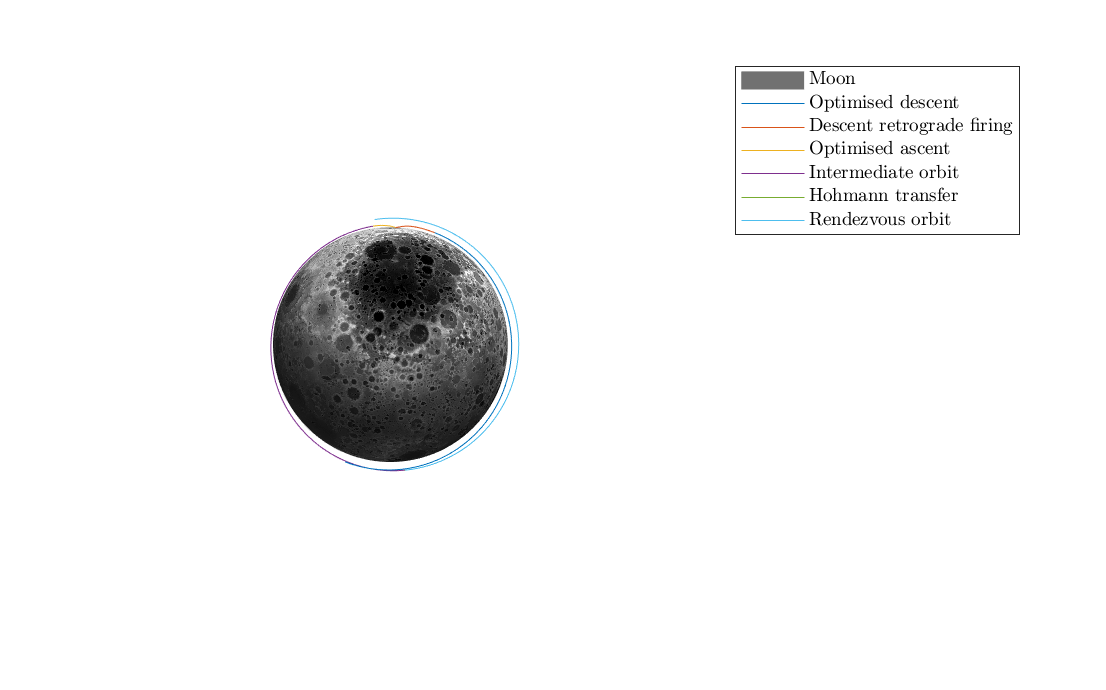
\includegraphics[height=\textheight]{optimisedTraj.eps}
  \caption{Simulated Apollo 11 Trajectory}
  \end{figure}
  \end{frame}
\begin{frame}{Other Cool Stuff}
\centering
    \includemedia[
    label=diceA,
    width=\textwidth,height=0.75\textheight,
    activate=pageopen,deactivate=pageclose,
  ]{}{MUGSMUGs.U3D}
\end{frame}
\section{I'm interested! How do I start learning?}
\begin{frame}{Programs/Compilers}
\begin{description}
\item[MikTex] Standalone \LaTeX compiler and editor. Good for local installations on Windows.
\begin{itemize}
\item Very easy to use
\item Good package support from CTAN (Comprehensive TeX Archive Network)
\item Not the prettiest
\item THE WHITE - IT BURNS
\end{itemize}
\onslide<2->\item[Overleaf] Web based, cloud storage. The \alert{Google Docs} of \LaTeX.
\begin{itemize}
\item Very easy to use
\item GitHub integration
\item Free Pro+ account by registering as a USYD student/staff member
\item Multiple author editing
\item Some packages might not be recognisable
\end{itemize}
\end{description}
\end{frame}
\begin{frame}
  \centering
We'll be using \alert{Overleaf}\\
\texttt{overleaf.com}
\end{frame}
\begin{frame}{Starting off a Document}
\begin{description}
\item[Define document class:]\hfill\\ \vspace{0.5cm}\texttt{{\textbackslash}documentclass[12pt]\{article\}}\hfill\\ \vspace{1cm}
\item[Begin document:]\hfill\\\vspace{0.5cm}
\texttt{{\textbackslash}begin\{document\}\hfill\\
\vspace{0.5cm}
<insert document content here>\hfill\\
\vspace{0.5cm}
{\textbackslash}end\{document\}}
\end{description}
\end{frame}
\begin{frame}
\centering
\large{Well done! You've just told \LaTeX\text{ }to create a new, blank document!\\
So... is that it?}
\end{frame}
\begin{frame}
\centering
\Huge{Not in the slightest!}
\end{frame}

\begin{frame}{The Preamble}
Everything before \texttt{{\textbackslash}begin\{document\}} is known as the \alert{preamble}. Let's start customising this.
\end{frame}

\begin{frame}[fragile]
  \begin{center}
  \Large{\begin{lstlisting}
  \documentclass{article}
  \title{My Title}
  \author{My Name}
  \date{\today}
  \begin{document}
  \maketitle
  ...
  \end{document}
  \end{lstlisting}}
\end{center}
\end{frame}
\begin{frame}[fragile]{Sections}
  \begin{center}
  \Large{\begin{lstlisting}
  \documentclass{article}
  \title{My Title}
  \author{My Name}
  \date{\today}
  \begin{document}
  \maketitle
  \section{My Section Name}
  ...
  \end{document}
  \end{lstlisting}}
\end{center}
\onslide<2->Bonus: try adding \verb|\makecontents| after \verb|\maketitle|
\end{frame}
\begin{frame}[fragile]{Maths}
Maths can be added pretty easily:
\begin{itemize}
  \item<1-> \verb|$\tan\alpha$| gives $\tan\alpha$
  \item<2-> \small{\verb|\[\int_{-\infty}^\infty \frac{\cos x}{x^2+1} dx = \frac{\pi}{e}\]| gives} \[\int_{-\infty}^\infty \frac{\cos x}{x^2+1} dx = \frac{\pi}{e}\]
\end{itemize}
\onslide<3-> Maths also comes in environments:\\
E.g. \verb|\begin{equation}...\end{equation}|
  \begin{equation}
   \frac{\dd \sin x}{\dd \cos x} = -\cot x
  \end{equation}
\onslide<4-> and \verb|\begin{align*}...\end{align*}|
  \begin{align*}
  F(s)&= \mathcal{L}\{t\}\\
  &= \frac{1}{s}
  \end{align*}
\end{frame}
\begin{frame}[fragile]{Packages}
  You'll notice that \verb|align*| doesn't work. The reason is, you haven't added the package necessary yet.\\
  Try including \verb|\usepackage{amsmath}| in your preamble.\hfill\\
  \vspace{3cm}
\onslide<2->  After you've checked that works - load the \verb|graphics| package.
\end{frame}
\begin{frame}[fragile]{Pictures}
  \begin{lstlisting}
  \begin{figure}[h!]
    \includegraphics{/path/to/figure}
    \caption{}
    \label{}
  \end{figure}
\end{lstlisting}
\onslide<2->The \verb|[h!]| component tells \LaTeX \text{ }to put the image exactly where you told it to. A big one-up on Word.
\end{frame}
\begin{frame}
  Congratulations! You've just learnt \LaTeX to the stage where you can do what Word does. But there is so much more!
\end{frame}
\begin{frame}{The best way to keep learning}
There is thousands of packages for different things! The only way you can learn them is by going through and using them in documents. \alert{Stackexchange is your friend}.\\
\vspace{1cm}
\onslide<2->The best way of continuing to learn \LaTeX \text{ }is to \alert{keep using it}. We've only touched the tip of the iceberg as to what \LaTeX \text{ }can do!\\
\vspace{1cm}
\onslide<3->Other things you can have \LaTeX \text{ }do:
\begin{itemize}
  \item<4-> Solve differential equations
  \item<5->  Plot natively in the document
  \item<6->  Presentations (like this one!)
\end{itemize}
\end{frame}
\section{Other programs to help create nice looking documents in \LaTeX}
\begin{frame}
  \begin{description}
    \item[TikzEdt]<1-> Semi-graphical tikz editor - very similar to the semiconductor drawing I showed earlier
    \item[gnuplot]<2-> Did those very nice plots earlier
    \item[MATLAB]<3-> You can change labels/figure ticks so they look like they're native to \LaTeX. \alert{Extremely} good integration
    \item[ImageMagick]<4-> Handy command line image editor
  \end{description}
\end{frame}
\begin{frame}
  \begin{columns}[c]
      \begin{column}{.5\textwidth}
        \vfill
       Jack Naylor\\
       jack.naylor@sydney.edu.au
       \vfill
      \end{column}
      \begin{column}{.5\textwidth}
\adjincludegraphics[height=1.3\textheight,trim={{.225\width} 0 {.25\width} 0},clip]{floor}
      \end{column}
    \end{columns}
\end{frame}

\end{document}
